\documentclass[12pt]{article}

% Encoding and fonts
\usepackage[utf8]{inputenc}      % Allow UTF-8 input
\usepackage[T1]{fontenc}         % Use modern font encoding
\usepackage{lmodern}             % Latin Modern fonts

% Page layout and spacing
\usepackage{geometry}
\geometry{letterpaper, margin=1in}
\usepackage{setspace}
\onehalfspacing                % Set line spacing to 1.5 for easier reading
\usepackage{parskip}           % Better paragraph spacing

% Microtypography for improved appearance
\usepackage{microtype}

% Hyperlinks
\usepackage{hyperref}
\hypersetup{
    colorlinks=true,
    linkcolor=blue,
    urlcolor=blue,
    citecolor=blue
}

% Header and footer customization
\usepackage{fancyhdr}
\pagestyle{fancy}
\fancyhf{} % clear all header and footer fields
\lhead{\textit{Book Reviews}}
\rhead{Perry Santry}
\cfoot{\thepage}

% Section formatting
\usepackage{titlesec}
\titleformat{\section}{\Large\bfseries}{\thesection}{1em}{}

% Graphics (if needed)
\usepackage{graphicx}
\usepackage{float}

% Optional: Bibliography support (if you wish to include references)
\usepackage[style=authoryear]{biblatex}
\addbibresource{references.bib}

% Custom commands for styling
\newcommand{\booktitle}[1]{\textbf{\textit{#1}}} % e.g., \booktitle{The Great Gatsby}
\newcommand{\review}[1]{\textit{#1}}              % e.g., \review{A captivating read...}

% Document metadata
\title{
    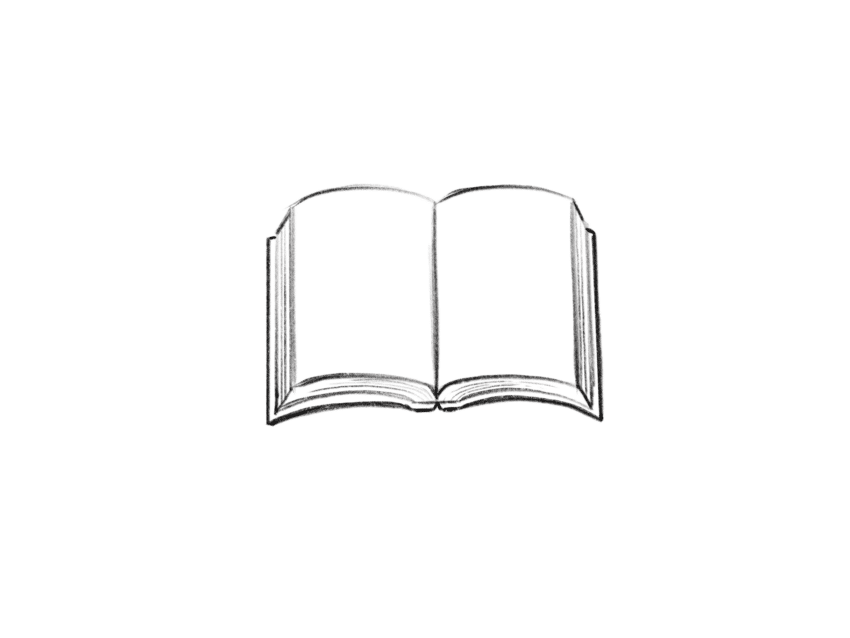
\includegraphics[width=0.55\textwidth]{bookimage.png} \\ 
    \textbf{\Huge Book Reviews} \\
    \large
    \date{}
}
\author{Perry Santry}

% End of preamble
\begin{document}
\vfill
\maketitle
\vfill
\thispagestyle{empty}
\newpage

\section*{}
\vfill
\Large{\textbf{As to why,}}
\\ \\
Unfortunately for myself, I never read much as a child. I found myself spending all my 
time with video games and television, as kids normally do nowaday, not caring for the 
story in the pages. This is not me saying I am done with that life, that would mean no 
longer being myself. However, I hope this article serves as a motivator and constant 
reminder to read and explore, feel what's in the pages, and digest thoroughly your 
thoughts on other peoples thoughts. You will notice I clearly have a favourite, but 
please don't take that to mean I am biased. I hope my reviews are as enjoyable as the 
books themselves.
\begin{flushright}
    - Perry Santry
\end{flushright}
\vfill

\thispagestyle{empty}
\normalsize
% Your reviews start here
\newpage
\tableofcontents
\setcounter{page}{1}  
\newpage
\section*{\booktitle{The Dark Tower IV: The Wizard and Glass}; \textbf{10/10}}
\addcontentsline{toc}{section}{The Dark Tower IV: The Wizard and Glass}
\review{The book starts off with the thrilling encounter between our ka-tet and Blaine the Mono. 
As usual, King does an incredible job at bringing your mind to a very chaotic place as we think 
this could be the end of Roland, Eddie, Susannah, Jake, and even Oy, death by suicidal train. 
Eddie Dean saves the day with a witty (practically impossible) riddle, that even Blaine the Mono 
couldn't solve. Thus, the ka-tet lived to see another Kansas, one that had been plagued with a 
very deadly disease. Here is where they find the thinny, here is where they learn the tale of Roland's 
first quest, here is where they hear the story of the Wizard's Glass. Roland decides that before they 
proceed on with their destiny of the Dark Tower, they must hear the story of what brought Roland here 
in the first place.} 
\\
This is why \textbf{The Dark Tower IV} is so incredible. The story of Roland becoming a Gunslinger is 
such an important part of the series as a whole, and finally getting this part of Roland's character 
feels like a vast emptiness has been filled. In the afterword, King tells of how difficult this 
story was to write, He had to make sure everything was perfect; the emotions a mature 14 year old boy 
would feel after leaving home for the first time with his two best friends on a quest that could cause 
or prevent the fall of Gilead. What King accomplishes within these 800 pages or so (depending on your 
version) is exactly that, \textit{perfection}.  

% More sections/reviews

\end{document}